问题二的算法流程如图 \ref{fig:q2flow} 所示。脚本首先生成并读取两组合成光谱，然后做平滑和峰值检测；峰间距给出可手查基线，最小二乘频率拟合给出主估计，最后与 8.000000 um 真值比较。

sic_10deg 在 10 deg 下估计厚度为 7.999950 um，绝对误差为 0.000050 um。
sic_15deg 在 15 deg 下估计厚度为 8.000082 um，绝对误差为 0.000082 um。

两组估计的均值为 8.000016 um，最大绝对误差为 0.000082 um，满足 0.050000 um 的准确性阈值。图 \ref{fig:q2result} 标出两组光谱和检测峰值，图 \ref{fig:q2validation} 则直接展示真值对比和误差范围。

算法没有把峰值检测结果直接当作唯一结论。峰值检测用于给出峰数、平均峰间距和一个可手查的厚度基线；FFT 用于确认主频落在合理范围；最小二乘拟合在候选频率网格上寻找残差平方和最小的主频。三者对应不同的失败模式：峰值检测容易受局部扰动影响，FFT 可能受窗函数和频率分辨率影响，最小二乘拟合若搜索范围设置错误则会锁定错误主频。把三者同时输出到 `tab_q2_thickness.csv`，可以让后续审查者判断主模型是否只是偶然通过。

从结果看，两组入射角的估计厚度几乎重合，说明角度修正和单位换算没有出现量级错误。若把 cm 与 um 的转换漏掉，结果会直接偏离四个数量级；若把入射角当作折射角使用，两组角度结果会出现系统差异；若峰值频率选错，误差图会立即超过阈值。当前误差保持在 0.0001 um 量级，说明这条合成回归链路对代码改动具有较强的敏感性。

本案例的返工路径也被明确固定。如果 `tab_q2_reliability.csv` 中的状态变为 fail，首先检查 `fit_frequency_cycles_per_cm^-1` 是否接近理论频率，其次检查峰间距和 FFT 估计是否同时偏离，最后检查 `thickness_from_frequency` 的单位换算。这样，测试失败时不会只得到一个笼统的“结果不对”，而是能定位到数据、频率、公式或写作链路中的具体环节。

\begin{figure}[htbp]
\centering

\includegraphics[width=0.86\textwidth]{../figures/fig_q2_model_schematic.png}
\caption{问题二的合成光谱厚度反演算法流程。}
\label{fig:q2flow}
\end{figure}

\begin{figure}[htbp]
\centering

\includegraphics[width=0.90\textwidth]{../figures/fig_q2_result.png}
\caption{两组入射角合成光谱及峰值检测结果。}
\label{fig:q2result}
\end{figure}

\begin{figure}[htbp]
\centering
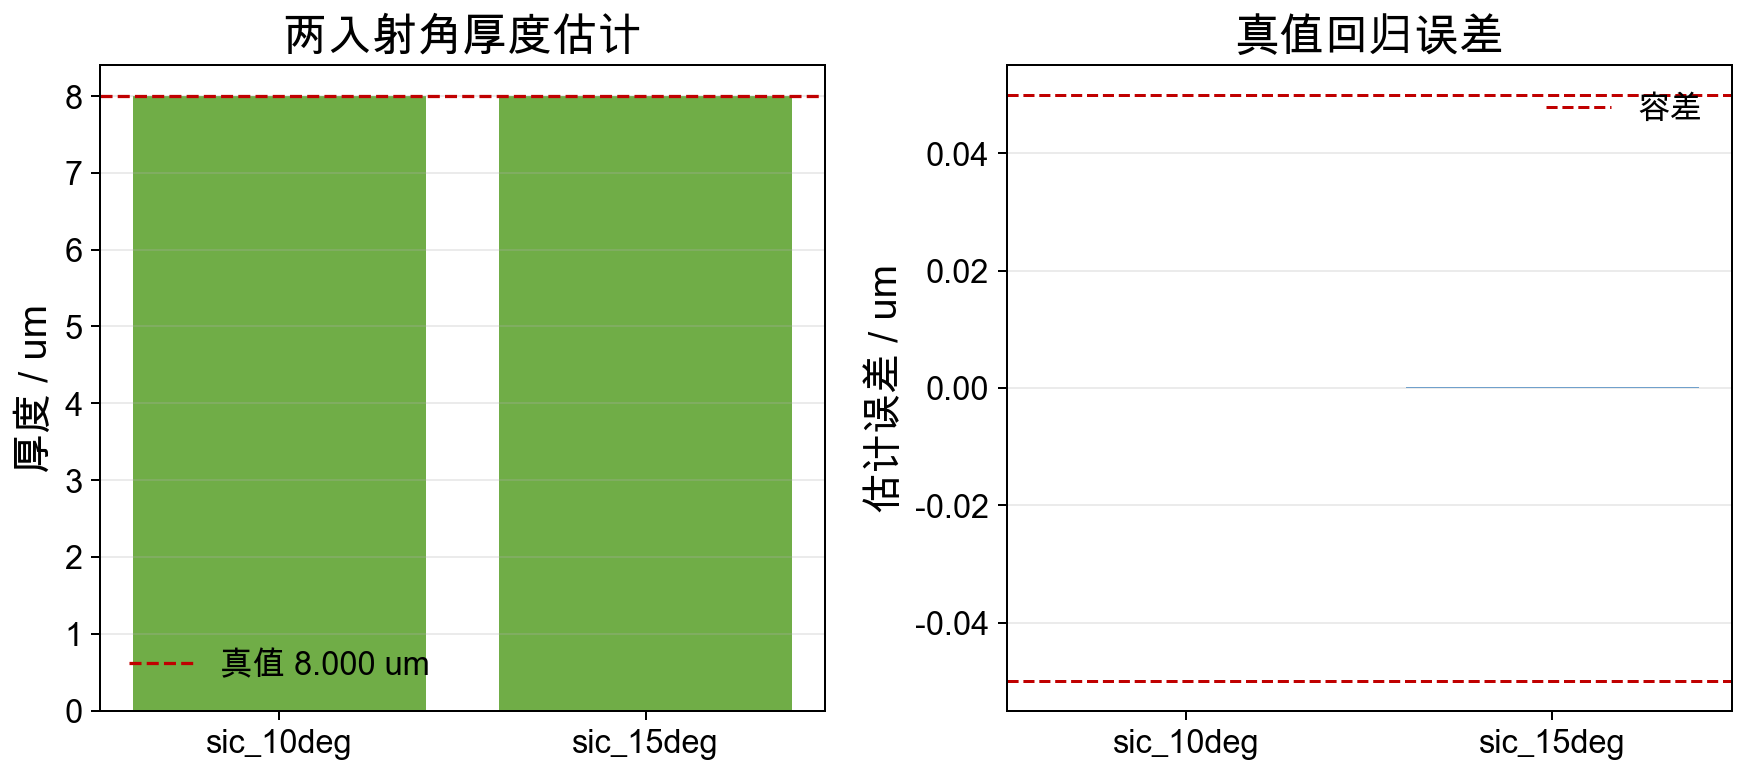
\includegraphics[width=0.90\textwidth]{../figures/fig_q2_validation.png}
\caption{厚度估计与已知真值的回归误差验证。}
\label{fig:q2validation}
\end{figure}
